%%%%%%%%%%%%%%%%%%%%%%%%%%%%%%%%%%%%%%%%%%%%%%%
%%%     Declarations (skip to Begin Document, line 88, for parts you fill in)
%%%%%%%%%%%%%%%%%%%%%%%%%%%%%%%%%%%%%%%%%%%%%%%

%%\documentclass[10pt]{article}
%%\documentclass[10pt]{report}
%%\documentclass[letterpaper]{article}
\documentclass[12pt]{article}
\usepackage{geometry}
%\usepackage{xcolor}
\usepackage[table]{xcolor}
\usepackage{amsmath}
\usepackage[some]{background}
%\usepackage{lipsum}
%\usepackage{natbib}
\usepackage[utf8]{inputenc} % set input encoding to utf8

% V E R S I O N I N G
\usepackage{vhistory}

% U N I T S
%\usepackage[binary-units]{siunitx}
\usepackage[]{siunitx}

% L I N E  N U M B E R S
\usepackage{lineno}
%\linenumbers
 
% C I T A T I O N S
%\usepackage[backend=biber,style=apa]{biblatex}
\usepackage[backend=biber, style=apa, maxcitenames=1]{biblatex} 
%\DeclareLanguageMapping{english}{english-apa}
%\usepackage{apacite}
%\bibliographystyle{apa}

%\usepackage{biblatex} 
\addbibresource{paperpile.bib}
\usepackage{datetime}

%\usepackage{hyperref}

% Tables
\usepackage{float}
\usepackage[utf8]{inputenc}
\usepackage{tabularx}
\usepackage{booktabs}
\usepackage{longtable}

\usepackage{diagbox} %table split headers
\usepackage{longtable}
\usepackage{array}
\usepackage{rotating}
\usepackage{eqparbox}
\usepackage{makecell, caption, booktabs}
\usepackage{tablefootnote}

\usepackage{colortbl}

% Confusion Table
\usepackage{rotating}
\usepackage{xparse}
\usepackage{booktabs, makecell, multirow}
\NewExpandableDocumentCommand\mcc{O{1}m}
    {\multicolumn{#1}{c}{#2}}
\usepackage{siunitx}

% W A T E R M A R K 
% This gets rid of the draft watermark on the title page
\backgroundsetup{contents={}}
%\usepackage[text=DRAFT]{draftwatermark}

% L I N E  S P A C I N G
%\renewcommand{\baselinestretch}{1.5} 

% This does not have the effect I wanted, putting the caption at the bottom.
%\usepackage{caption}
%\captionsetup[table]{position=bottom} 

% Stuff needed to get table to span pages
\usepackage{enumitem}
%\usepackage{array, booktabs, longtable}
\newcolumntype{x}[1]{>{\raggedright}p{#1}}

\usepackage{etoolbox}
\AtBeginEnvironment{longtable}{%
    \setlist[itemize]{nosep,     % <-- new list setup
                      topsep     = 0pt       ,
                      partopsep  = 0pt       ,
                      leftmargin = *         ,
                      label      = $\bullet$ ,
                      before     = \vspace{-\baselineskip},
                      after      = \vspace{-0.5\baselineskip}
                        }
                           }% end of AtBeginEnvironment
% End table span

\definecolor{green}{rgb}{0.1,0.1,0.1}
%\color{green!40!yellow})

\newcommand{\done}{\cellcolor{teal}done}  %{0.9}
\newcommand{\hcyan}[1]{{\color{teal} #1}}

% Listings
\usepackage{listings}

\usepackage{geometry}  % Lots of layout options.  See http://en.wikibooks.org/wiki/LaTeX/Page_Layout
\geometry{letterpaper}  % ... or a4paper or a5paper or ... 
\usepackage{fullpage}  % somewhat standardized smaller margins (around an inch)
\usepackage{setspace}  % control line spacing in latex documents
\usepackage[parfill]{parskip}  % Activate to begin paragraphs with an empty line rather than an indent

\usepackage{amsmath,amssymb}  % latex math
\usepackage{empheq} % http://www.ctan.org/pkg/empheq
\usepackage{bm,upgreek}  % allows you to write bold greek letters (upper & lower case)

% for typsetting algorithm pseudocode see http://en.wikibooks.org/wiki/LaTeX/Algorithms_and_Pseudocode
\usepackage{algorithmic,algorithm}  

\usepackage{graphicx}  % inclusion of graphics; see: http://en.wikibooks.org/wiki/LaTeX/Importing_Graphics
% allow easy inclusion of .tif, .png graphics
\DeclareGraphicsRule{.tif}{png}{.png}{`convert #1 `dirname #1`/`basename #1 .tif`.png}

% \usepackage{subfigure}  % allows subfigures in figure
\usepackage{caption}
\usepackage{subcaption}

\usepackage{xspace}
\newcommand{\latex}{\LaTeX\xspace}

\usepackage{color}  % http://en.wikibooks.org/wiki/LaTeX/Colors

\long\def\todo#1{{\color{red}{\bf TODO: #1}}}

\long\def\ans#1{{\color{blue}{\em #1}}}
\long\def\ansnem#1{{\color{blue}#1}}
\long\def\boldred#1{{\color{red}{\bf #1}}}
\long\def\boldred#1{\textcolor{red}{\bf #1}}
\long\def\boldblue#1{\textcolor{blue}{\bf #1}}

% Useful package for syntax highlighting of specific code (such as python) -- see below
\usepackage{listings}  % http://en.wikibooks.org/wiki/LaTeX/Packages/Listings
\usepackage{textcomp}


%%% The following lines set up using the listings package
\renewcommand{\lstlistlistingname}{Code Listings}
\renewcommand{\lstlistingname}{Code Listing}

%%% Specific for python listings
\definecolor{gray}{gray}{0.5}
\definecolor{green}{rgb}{0,0.5,0}

\lstnewenvironment{python}[1][]{
\lstset{
language=python,
basicstyle=\footnotesize,  % could also use this -- a little larger \ttfamily\small\setstretch{1},
stringstyle=\color{red},
showstringspaces=false,
alsoletter={1234567890},
otherkeywords={\ , \}, \{},
keywordstyle=\color{blue},
emph={access,and,break,class,continue,def,del,elif ,else,%
except,exec,finally,for,from,global,if,import,in,i s,%
lambda,not,or,pass,print,raise,return,try,while},
emphstyle=\color{black}\bfseries,
emph={[2]True, False, None, self},
emphstyle=[2]\color{green},
emph={[3]from, import, as},
emphstyle=[3]\color{blue},
upquote=true,
morecomment=[s]{"""}{"""},
commentstyle=\color{gray}\slshape,
emph={[4]1, 2, 3, 4, 5, 6, 7, 8, 9, 0},
emphstyle=[4]\color{blue},
literate=*{:}{{\textcolor{blue}:}}{1}%
{=}{{\textcolor{blue}=}}{1}%
{-}{{\textcolor{blue}-}}{1}%
{+}{{\textcolor{blue}+}}{1}%
{*}{{\textcolor{blue}*}}{1}%
{!}{{\textcolor{blue}!}}{1}%
{(}{{\textcolor{blue}(}}{1}%
{)}{{\textcolor{blue})}}{1}%
{[}{{\textcolor{blue}[}}{1}%
{]}{{\textcolor{blue}]}}{1}%
{<}{{\textcolor{blue}<}}{1}%
{>}{{\textcolor{blue}>}}{1},%
%framexleftmargin=1mm, framextopmargin=1mm, frame=shadowbox, rulesepcolor=\color{blue},#1
framexleftmargin=1mm, framextopmargin=1mm, frame=single,#1
}}{}
%%% End python code listing definitions

\DeclareMathOperator{\diag}{diag}
\DeclareMathOperator{\cov}{cov}


%\bibliography{./paperpile.bib}
%\author{Evan McGinnis}
%\title{Automated Weeding}



\definecolor{titlepagecolor}{cmyk}{1,.60,0,.40}

\DeclareFixedFont{\bigsf}{T1}{phv}{b}{n}{1.5cm}

\backgroundsetup{
scale=1,
angle=0,
opacity=1,
contents={\begin{tikzpicture}[remember picture,overlay]
 \path [fill=titlepagecolor] (-0.5\paperwidth,5) rectangle (0.5\paperwidth,10);  
\end{tikzpicture}}
}
\makeatletter                       
\def\printauthor{%                  
    {\large \@author}}              
\makeatother
\author{%
\setstretch{1.0}
    Evan McGinnis \\
    PhD Student \\
    Student ID\#  23633780\\
    Biosystems Analytics \\
    \today \\
    \texttt{evanmc@arizona.edu}\vspace{40pt} \\
    }

\begin{document}

\begin{titlepage}
\BgThispage
\newgeometry{left=1cm,right=4cm}
\vspace*{1cm}
\noindent
%%\vspace*{0.4\textheight}
\textcolor{white}{\Huge\textbf{\textsf{Classification of weed and crop vegetation in lettuce field}}}
\vspace*{2.5cm}\par
\noindent
\begin{minipage}{0.35\linewidth}
    \begin{flushright}
        \printauthor
    \end{flushright}
\end{minipage} \hspace{15pt}
%
\begin{minipage}{0.02\linewidth}
    \rule{1pt}{175pt}
\end{minipage} \hspace{-10pt}
%
\begin{minipage}{0.8\linewidth}
\vspace{5pt}
    \begin{abstract} 
\setstretch{1.0}
This paper proposes a study of classification of vegetation found within a lettuce field at various heights AGL. While there are generally two categories of vegetation encountered within a field: weed and crop, these categories do not quite connote the fate of the vegetation. \textit{Desired} and \textit{undesired} might be names that more accurately describe their fate. This study will examine the classification of images acquired close to ground level (such as would be acquired from a tractor-towed system) as well as images acquired from unmanned aerial vehicle flights at various altitudes.
    \end{abstract}
\end{minipage}
\end{titlepage}
\restoregeometry
%
% F R O N T  M A T T E R
%
{
\setstretch{1.0}
\tableofcontents
\listoftables
\listoffigures
\newpage
}

{
\setstretch{1.0}
\begin{versionhistory}
  \vhEntry{1.0}{4 May 2023}{EM}{Initial revision}
\end{versionhistory}
\newpage
}

%
% B E G I N   T E M P L A T E   F R O M   W O R D
%

%
% O V E R V I E W
%

\section{Overview}
\label{section:proposal}
This study will produce a system capable of classifying vegetation and formation of a treatment plan suitable for precision treatment in near real-time under field conditions.  Previous attempts at classification took the approach of classifying images obtained in the field using compute power in a centralized data center. Instead, image processing and subsequent classification will be done in-situ on the same platform as the image acquisition.  In this system, images are processed and treatment plans are formed as images are acquired. Images and other data about the vegetation are gathered by two different platforms: terrestrial and aerial. Terrestrial platforms include both images acquired manually with hand-held cameras and images gathered via tractor-towed solutions. The aerial image acquisition platform is used for heights above the level for terrestrial applications, usually above 1 meter.


\section{Introduction}
This study will use morphological and color features to distinguish between crop and weeds, and weeds will be the target of subsequent treatment. There are three challenges that warrant attention here: separation of vegetation from background, feature extraction, and weed/crop discrimination,\\
Aspects of this problem are well researched and documented. \citeauthor{Hamuda2016-dw} surveys the task of separation of vegetation and non-vegetated portions of visible light images, and that work will be used in this proposal \parencite{Hamuda2016-dw}. The disadvantages mentioned in that study of color-index based schemes, most notably changing lighting conditions leading to inconsistent results, and the expected dominant color of vegetation is green, will not be of concern for this work. Tractor-towed systems may feature enclosures that block all ambient light and use controlled lighting during image acquisition, but this will not be the case in images acquired with UAVs and is typically not encountered with images acquired manually.\\
There are two types of features to be considered: color and structural. \citeauthor{Sabzi2020-af} studies both of these feature types in a study of weed identification in a potato field \parencite{Sabzi2020-af}. Color feature evaluation was carried out in \textit{transformed} color spaces: Hue, Saturation, Intensity (HSI); Hue, Saturation, Value (HSV); Luminance, In-Phase, Quadrature (YIQ); and Luminance, blue - luminance, and red - luminance (YCbCr). Structural features were not heavily emphasized in this model, as the area-to-length ratio was the sole structural component considered. While the correct classification rate in that study exceeded 98\%, the field tests showed a commercially nonviable speed of 0.15 m/s. \footnote{The article detailing the study does not include sufficient details to form a theory on why the speed achieved is so slow. While illustrations indicate that image processing is executed with Matlab on a laptop, details of those components are missing.} \\
Lin, in a study of corn and weed species identification, identifies key shape features, along with formulae for their determination that can then be exploited in discrimination: shape index and length-to-width ratio \parencite{Lin2017-xq}. Wirth, in a presentation on shape analysis, details aspects of (and formulae for) structural features of objects. Among these are: roundness, convexity, solidity, elongation, and compactness \parencite{Wirth2004-li}.\\
Using both color and morphological features it is possible to achieve both the speed and accuracy required in weed identification. While research has shown that distinguishing crop from weeds is possible given sufficient computing resources, doing so in a field setting with limited computational power and at speeds considered commercially viable is not fully addressed. Coupling an image recognition system to a treatment system is often left as a exercise for the reader or mentioned as a possible application. This study will provide a complete solution.


\subsection{Results}
Analysis of a set of visible-light images\footnote{Image set of lettuce beds supplied by Dr. Mark Siemens, University of Arizona} shows that the general concepts of using a few features for object classification is viable (refer to Table~\ref{fig:learning}).

{\renewcommand{\arraystretch}{2}%
\begin{table}[H]
	\centering
   	 \begin{tabular}{  l  p{4cm}  p{5cm} }
        	\toprule
		\textbf{Method}      
		& \textbf{Train}   
		& \textbf{Test} \\\midrule
		Logistic Regression
		& 0.9790       
		& 0.9787 \\\hline
		KNN     
		& $1.0$                    
		& $0.86$ \\\hline
		Decision Tree
		& 1.0
		& 0.96 \\\hline
		Boosted Gradient     
		& 1.0
		& 0.957 \\\hline
		Random Forest      
		& 1.0
		& 0.986 \\\hline
		Support Vector
		& 0.989
		& 0.971 \\\hline
       	 \bottomrule
	\end{tabular}
    	\caption[Various Machine Learning Algorithms]{Results of using various machine learning algorithms for weed recognition}
 	 \label{fig:learning}
\end{table}

These results reflect the use of four attributes of each plant in the image:
\begin{itemize}
	\item{Length/Width Ratio, }
	\item{Shape Index, an expression of how 'rough' the edges of the object are}
	\item{YIQ In-phase mean, a measure of the average after a colorspace transformation}
	\item{Normalized distance from the crop line, as weeds are often more distant from the crop line than are crop}
\end{itemize}

The image set used in this analysis had these characteristics:\footnote{\url{https://data.cyverse.org/dav-anon/iplant/home/evanmc/lettuce-images.zip}}
\begin{itemize}
	\item{Captured using a Samsung SM-G930V cameraphone}
	\item{Taken at Yuma Research Center, Yuma AZ}
	\item{Captured 18 Jan 2019}
	\item{Captured using ambient light}
	\item{2880x2160 pixels}
\end{itemize}

While encouraging, it is important to keep two points in mind when considering these results: 
\begin{itemize}
	\item{These results are for an image set taken at only a single point in the growth cycle. It may be the case that both color and morphological features of the vegetation may change over the development cycle. Models trained using images from one point in the cycle may not be as accurate when presented with images taken an a different point}
	\item{Misclassification of a weed as a crop, while not optimal, does not have direct costs in terms of marketable crop. Mis-identified weeds are simply not treated. Misclassification of crop as weed has very direct costs, as marketable crop is mistakenly targeted for treatment, a mistake that has  monetary costs.}
\end{itemize}

As shown in Table~\ref{table:confusion}, we can see the cost of making an error.}

%
% C O N F U S I O N  M A T R I X
%
 \begin{table}[ht]
    \renewcommand{\arraystretch}{1.3}
    \footnotesize
    \setlength{\tabcolsep}{0pt}
	\settowidth\rotheadsize{Predicted}
    	\centering

	%\begin{tabular*}{\linewidth}{@{\extracolsep{\fill}}lc| *{2}{S[table-format=2.2]}| S[table-format=2.2]}
	\begin{tabular*}{0.55\linewidth}{@{\extracolsep{\fill}}lc| *{2}{S[table-format=2.2]} | S[table-format=2.2]}
    		\hline\hline
   		\multicolumn{2}{l|}{}   &   \multicolumn{2}{c|}{Actual}                            \\
   		\multicolumn{2}{c|}{}    & {Crop} & {Weed\ \ }  & {\bfseries Precision}\\ 
    		\hline
		\multirow{2}{*}{\rothead{\ \ \ \ \ Pred.}} 
    			& Crop   & 28 &  2 &  .93   \\
    			& Weed  & 6  & 201 &  .97\\
    		\hline
 		& \bfseries Recall\ \ 
        	& \textbf{.82}         & .99         &           \\ 
    		\hline\hline
	\end{tabular*}
	\caption[Confusion matrix for KNN]{In this confusion matrix for KNN, we can see that the misclassification of crop as weed drives the \textit{recall} metric to 82\%}
	\label{table:confusion}

% When we had only one table
\end{table}

 \begin{table}[ht]
    \renewcommand{\arraystretch}{1.3}
    \footnotesize
    \setlength{\tabcolsep}{0pt}
	\settowidth\rotheadsize{Predicted}
    	\centering
	%\begin{tabular*}{\linewidth}{@{\extracolsep{\fill}}lc| *{2}{S[table-format=2.2]}| S[table-format=2.2]}
	\begin{tabular*}{0.55\linewidth}{@{\extracolsep{\fill}}lc| *{2}{S[table-format=2.2]} | S[table-format=2.2]}
    		\hline\hline
   		\multicolumn{2}{l|}{}   &   \multicolumn{2}{c|}{Actual}                            \\
   		\multicolumn{2}{c|}{}    & {Crop} & {Weed\ \ }  & {\bfseries Precision}\\ 
    		\hline
		\multirow{2}{*}{\rothead{\ \ \ \ \ Pred.}} 
    			& Crop   & 28 &  5 &  .85   \\
    			& Weed  & 5  & 199 &  .98\\
    		\hline
 		& \bfseries Recall\ \ 
        	& \textbf{.85}         & .98         &           \\ 
    		\hline\hline
	\end{tabular*}
	\caption[Confusion matrix for Logistic Regression]{In this confusion matrix for Logistic Regression, we can see that the \textit{recall} is much closer for both KNN and Logistic Regression approaches than the overall accuracy values presented earlier.}
	\label{table:confusion}
\end{table}

%
% D I S C U S S I O N
%


\subsection{Discussion and Conclusion}
These results show that it is possible to distinguish crop and weed in visible light images with one important caveat: the results reflect only a specific point in the development cycle. The shape or color of the crop may vary with time, so careful consideration must be made to the consistency of these features over time. Overall accuracy cannot be used as the sole metric when evaluating the performance of the learning approaches. Logistic Regression, for instance, has a much higher overall accuracy than does KNN, but using KNN yields much closer recall.  If we consider only the high-cost (monetarily) error, the two approaches are actually quite close.

%Do not use abbreviations or insert tables, figures or references into your abstract. You abstract generally should not exceed about 300 words. 
 
 \newpage

%
% P R O B L E M
%
 
\section{Problem Statement}
Crop rows contain two sets of unwanted vegetation: marketable crop and undesired vegetation in the form of misplaced crop and weeds. Consider the row of lettuce illustrated by Figure~\ref{fig:weed-placement}. In these images the row contains weeds within the row itself (inter-row) and weeds not within the row. An additional complication seen in the inter-row example is that the weed is within close proximity to the crop. \\
In Arizona, approximately 45,000-55,000 acres of lettuce are grown, with 95\% of that figure produced in Yuma County, the location of this study \parencite{Kerns1999-la}.

Treatment of unwanted vegetation is executed using a high speed centimeter scale resolution sprayer already developed \parencite{Siemens2020-ds}, but vegetation targeted for elimination must not be \textit{too} close to the crop in order to avoid inadvertent damage.

\begin{figure}[H]
	\centering
	\begin{subfigure}[]{.40\textwidth}
		\includegraphics[width=1\linewidth]{./figures/weed-outside-row.jpg}
		\caption{A row of lettuce with weed outside the crop row}
		\label{fig:lettuce-row-with-weed-outside}
	\end{subfigure}
	\begin{subfigure}{.40\textwidth}
		\centering
		\includegraphics[width=1\linewidth]{./figures/weed-within-row.jpg}
		\caption{A row of lettuce with weed within the crop row}
		\label{fig:lettuce-row-with-weed-inside}
	\end{subfigure}
	\caption[Two cases of weed placement]{Two cases of weed placement}
	\label{fig:weed-placement}
\end{figure}


\subsection{Overview}

\subsection{Research Question/Hypothesis}
This study will seek the answers to three related questions:
\begin{enumerate}
\item{Is it possible to distinguish weeds from crop in visible light images?}
\item{Is it possible to make such a distinction in the time required to support a commercially viable speed of treatment?}
\item{Are the features used to make the distinction invariant over the growing season?}
\end{enumerate}

The first question is a more basic, but essential one. We are considering using only a subset of the features of objects withing a visible light image. Can the two sets of vegetation be distinguished using a subset of these attributes?
\begin{itemize}
	\item{Structural Features}
	\begin{itemize}
		\item{Distance to cropline, as weeds tend to be outside the crop}
		\item{Total leaf area}
		\item{Shape Index, the relationship between an object's perimeter and area}
		\item{Features in HSI, HSV, YIQ, and YCbCr color spaces}
		\item{Elongation, the ratio of length to width of the bounding box of an object}
		\item{Eccentricity, the ratio of the length of an object's minor axis to its major axis}
		\item{Solidity, the ratio of an object's area to its convex area}
		\item{Convexity, the ratio of an object's convex perimeter to its perimeter}
		\item{Compactness, the ratio of an object's area to a circle with the same perimeter}
		\item{Length to width ratio, the ratio of the maximum eigenvector to the minimum eigenvector of the covariance matrix of the perimeter's (x,y) coordinates}
		\item{Size Ratio}
	\end{itemize}
	\item{Color Features}
	\begin{itemize}
		\item{Components of HSI color-space}
		\item{Components of HSV color-space}
		\item{Components of YIQ color-space}
	\end{itemize}
\end{itemize}

While it should be possible to distinguish the two sets of vegetation using these features given enough computing power, is it possible to do so in real time with compute power that is available in the field? Inexpensive Graphic Processing Units (GPUs) are commonly used in machine learning problems such as these, and a key part of this study will be to assess the applicability of this technology for the problem space. Achieving a target speed of a forward progress rate of 4 kph (or 2.49 mph.  A speed of 2 mph was used in \citeauthor{Siemens2020-ds}'s study for the high precision spray unit [\cite{Siemens2020-ds}].) sets the bounds on a compute time budget. The camera will be placed 17 inches (0.43 m) above the crop bed. Given an example camera with an 8mm focal length lens, an image size of 23 cm x 13 cm can be obtained.\footnote{Specifications for Basler 1920-25g camera were used in these calculations. That specific model is no longer produced, but the specifications will suffice for this case} In one second, the system must be capable of processing 4.82 images, giving a time budget of around 208 milliseconds per image to perform two tasks: distinguish between crop and weed, and form a treatment plan. While the exact numbers in the final system will deviate from those presented here, these frame the discussion and set a target processing speed.

While much of the work discussed thus far has involved the mechanisms used to distinguish crop from weeds, the image processing workflow involves more steps that have not yet been discussed in detail. The overall workflow is outlined in Figure~\ref{fig:image-processing-workflow}
\begin{figure}[H]
	\centering
	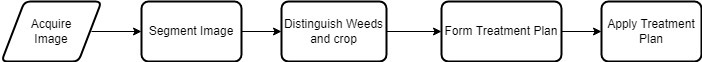
\includegraphics[width=0.75\linewidth]{./figures/image-processing-workflow.jpg}
	\caption{Image processing workflow}
	\label{fig:image-processing-workflow}
\end{figure}

%This workflow shows a crucial step

 %\newpage
 
\section{Objective and Aims}
The objective of this study is to not only answer the questions identified in the previous section, but to produce a viable system for field deployment. 

\subsection{Specific Aims}
The aims of this study will be to solve several problems in addition to the key questions posed earlier:
\begin{itemize}
	\item{Survey and develop image segmentation techniques that operate in the lighting conditions encountered in field conditions}
	\item{Develop machine learning approaches to discriminate between crop and weed that operate within the targeted time budget}
	\item{Design and integrate a system that will incorporate all aspects of the workflow shown in Figure~\ref{fig:image-processing-workflow}}
\end{itemize}
\newpage

%
% L I T E R A T U R E  R E V I E W 
%

\section{Background and Significance}

%\subsection{Herbicide Exposure}
%Exposure to synthetic herbicides \cite{Rydz2021-ar}
\subsection{Image Segmentation}
Humuda discusses  algorithms to separate the vegetated portion of an image from non-vegetated portions \cite{Hamuda2016-dw}. Specifically, this review compares the efficacy of approaches based on color index in visible light images (Table~\ref{table:segmentation}). This paper details the formulae for various approaches. Hunt details an approach to segmentation that takes into account the responsiveness of the sensor \cite{Hunt2013-ih}.
{\renewcommand{\arraystretch}{2}%

{
% This avoids the document line spacing affecting the contents of the table
\setstretch{1.0}
% Example to span two pages
\begin{longtable}{x{\dimexpr.2\columnwidth-2\tabcolsep}
                  x{\dimexpr.4\columnwidth-2\tabcolsep}
                  x{\dimexpr.4\columnwidth-2\tabcolsep}}
%\begin{hyphenrules}{nohyphenation}
    \caption{Visible light indices}\label{tab:example}  \\
\toprule
{\textbf{Index}} & {\textbf{Formula}} & {\textbf{Comment}}
\tabularnewline
\midrule
    \endfirsthead
%%%%
    \caption{Visible light indices (cont.)}\label{tab:example}  \\
\toprule
{\textbf{Index}} & {\textbf{Formula}} & {\textbf{Comment}}
\tabularnewline
\midrule
    \endhead
%%%%
\midrule[\heavyrulewidth]
\multicolumn{3}{r}{\footnotesize\itshape
                   Continued on the next page}
    \endfoot
%%%%
\bottomrule
    \endlastfoot
%%%%
		Triangular Greenness
		& \begin{minipage}[t]{0.3\textwidth}
			$R_{green} - \alpha R_{red} - \beta R_{blue}\\ \alpha = \frac {2(\lambda_{blue} - \lambda_{green})} {(\lambda_{blue} - \lambda_{red})}\\ 
		    	\beta = \frac {2(\lambda_{green} - \lambda_{red})} {(\lambda_{blue} - \lambda_{red})} $
		   \end{minipage}     
		& Corrects for camera calibration using the peak sensitivity
\tabularnewline\addlinespace

		Normalized Difference     
		& $128 * \left( \left( \frac {(G - R)} {(G + R)} \right) + 1 \right) $                    
		& The NDI index produces a near-binary image. 
\tabularnewline\addlinespace

		Excess Green      
		& \begin{minipage}[t]{0.3\textwidth}
			$R = \frac {R} {R_{max}}\\ G = \frac {G} {G_{max}}\\ B = \frac {B} {B_{max}}$ 
		   \end{minipage}
		& ExG provided a clear contrast between plants and soil 
\tabularnewline\addlinespace

		Excess Red      
		& $1.3 R - G$ 
		& inspired by the fact that there are 4\% blue, and 32\% green, compared with 64\% red cones in the retina of the human eye
\tabularnewline\addlinespace

		Color Index of Vegetation Extraction      
		& $0.441 R - 0.811 G + 0.385 B + 18.78745$
		& This method was proposed to separate green plants from soil background in order to evaluate the crop growing status.
\tabularnewline\addlinespace

		Excess Green - Excess Red   
		& $ExG - ExR$ 
		& ExG used to extract the plant region and ExR used to eliminate the background noise (soil and residue) where green–red material (stems, branches, or petioles) may exist
\tabularnewline\addlinespace

		Normalized Green-Red Difference    
		& $\frac {(G - R)} {(G + R)}$ 
		& The method of NGRDI was used to overcome the differences in exposure settings selected by the digital camera when acquiring aerial photography of the field. 
\tabularnewline\addlinespace

		Vegetative Index      
		& $\frac {G} {R^aB^{(1-a)}}, a = 0.667$ 
		& VEG has a significant advantage because it is robust to lighting change.
\tabularnewline\addlinespace

		Com1   
		& $ExG + CIVE + ExGR + VEG$ 
		& High computational cost --- does not perform well in high or low light levels
\tabularnewline\addlinespace

		Modified Excess Green      
		& $1.262G - 0.884R = 0.311B$ 
		& Does not perform well in high or low light levels. 
\tabularnewline\addlinespace

		Combined Indices 2      
		& $0.36ExG + 0.47CIVE + 0.17VEG$ 
		& Uses weighting factors to emphasize strengths of various approaches
\tabularnewline\addlinespace

\tabularnewline\addlinespace
\label{table:segmentation}
\end{longtable}
}	
% End example
Otsu describes an approach to automatically select thresholds in images \cite{Otsu1979-io}. This technique is carried out on \textit{greyscale} images, not images with color information, so conversion to greyscale will be integrated into the image processing workflow. The technique is not particularly compute intensive, but details a mechanism for automatically choosing a threshold for segmentation, obviating the need for choosing this threshold manually. While the technique can indeed select a segmentation threshold, it tends to result in images that contain too much of the background. Subsequent processing of these images suffer from two problems: increased compute time (due to the presence of non-vegetated pixels) and the distortion of both shape and color feature computations.


%\end{longtable}
\subsection{Weed Identification}
In the proposed workflow, two sets of features are extracted from vegetation in the images: structural and color. Wirth gives an overview of the structural shape features used in this study: compactness, elongation, eccentricity, roundness, convexity and solidity \cite{Wirth2004-li}. 
Sabzi presents an analysis of factors for weed/crop discrimination that include both structural and color features \cite{Sabzi2020-af}. In that study, Sabzi identifies these features that produce a 98\% correct classification rate: saturation in the HSV \cite{Various_undated-yv} color space, the mean value of Hue in the HSI color space, the area to length ratio, the mean Chrominance component in the YCbCr \cite{Wikipedia_contributors2022-qd} color space, and the standard deviation of the in-phase component of the YIQ \cite{Various_undated-cz} color space.
Hemming studies using both morphological and color features, concluding that color features increase the accuracy of using morphological features alone. \cite{Hemming2001-ue} \\

 \citeauthor{Sabzi2020-af} employs both color and morphological features in crop/weed discrimination\parencite{Sabzi2020-af}:
\begin{itemize}
	\item{gray level co-occurrence matrix (GLCM)}
	\item{the standard deviation of saturation (S) component in HSV color space}
	\item{difference of first and seventh moment invariants}
	\item{mean value of hue component (H) in HSI color space} 
	\item{area to length ratio}
	\item{average blue-difference chrominance (Cb) component in YCbCr color space}
	\item{standard deviation of in-phase (I) component in YIQ color space}
\end{itemize}


\newpage
 
\section{System}
\label{section:system}

The system consists of three major subsystems: image processing, odometry, and treatment. Of these subsystems, only the image processing and odometry systems are covered in this study. The treatment sub-system has been developed separately \cite{Siemens2020-ds}, and will not be explored in-depth in this proposal. While treatment is important to the overall efficacy of the system, the realization of the treatment through mechanics, chemical, or other means (lasers) will not have significant bearing on this proposal. The image processing system uses machine learning to distinguish weed from crop and will direct treatment of vegetation deemed to be a weed, and represents the bulk of this proposal. 

The system will be realized as an integrated solution, towed behind a tractor, treating a single bed with two crop rows as it travels along the row.
\begin{figure}[H]
	\centering
	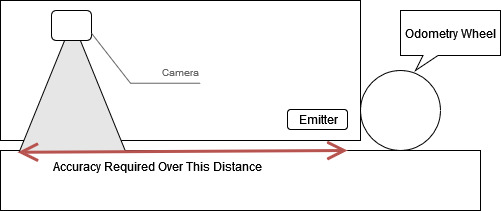
\includegraphics[width=0.4\linewidth]{./figures/system-in-field.jpg}
	\caption[An elevation view of the system in the field]{An elevation view of the system in the field --- the system depicted here is towed along a single bed, treating weeds as the system makes forward progress.}
	\label{fig:system-in-field}
\end{figure}

The integrated system is composed of four components:
\begin{itemize}
\item{A machine-vision camera, contained in a protective housing, and mounted on a gimbal system}
\item{An image processing system, where weeds within the images acquired by the camera and treatment plans formed}
\item{A controller, whose duties are to interpret signals from the odometry system and to direct the treatment/sprayer subsystem}
\item{A treatment subsystem, here, a high-precision sprayer}
\end{itemize}

Figure~\ref{fig:system-overview} illustrates how the system will be realized for a single-bed, two-row system. In this realization, some components are dedicated to a crop row (the camera and associated lighting) and some are shared as a central resource (the National Instruments RIO controller)
\begin{figure}[H]
	\centering
	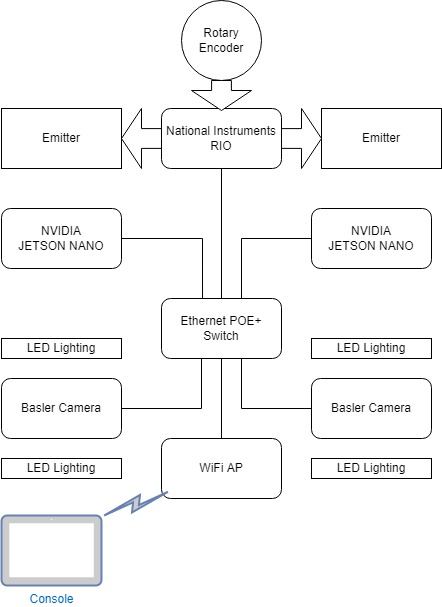
\includegraphics[width=0.4\linewidth]{./figures/system-overview.jpg}
	\caption[An overview of the system]{An overview of the system -- the system depicted here targets a single row, two crop-line crop bed}
	\label{fig:system-overview}
\end{figure}

\subsection{Data Management}
This proposal does not explicitly cover the fate of the data captured (images of vegetation) and treatment plans formed during operation, but it is anticipated that these items will be archived in a cloud (i.e., AWS) or research system (i.e., CyVerse), but the details of that are beyond the scope of this proposal. Those data can be used for two purposes:
\begin{itemize}
	\item{future work that does not involve real-time response, as well as the assessment of individual treatment sessions.}
	\item{evaluation of shape and color features across the growing season}
\end{itemize}
It is this second use that will be integrated in this study. The extent to which the color and shape features are invariant across the growing season may affect the efficacy of the weed/crop discrimination.

\subsection{Development Environment and Software Components}
The software development environment will consist of:
\begin{itemize}
	\item{Microsoft Windows 10}
	\item{PyCharm Python IDE version 2020.3}
\end{itemize}
It is not likely that the development environment will have any affect on the deployed product.  Development using different operating systems (Ubuntu, for example) may be used, but are not currently planned.
All software will be developed using Python 3.8 with these software components:
\begin{itemize}
	\item{eJabberd XMPP Server -- While no alterations to this server will be made apart from customized options, this server will provide a framework for all communications between physical components.  As this is a critical component, both the concepts behind XMPP and its use here will be discussed in detail below.}
	\item{Slix XMPP Client Library -- This client library will be used on all physical components to provide the connectivity to the XMPP server.}
	\item{Scikit-Learn -- This client library will be used to supply the machine-learning implementations used in this project.}
	\item{NumPy -- While early stages of this project will use NumPy to perform computations on data contained in images (particularly in image segmentation), the use of Numpy will be used only in the early stages of the project. As computation time becomes more critical, GPU programming libraries will be used instead to perform these calculations.}
	\item{National Instruments daqmx Python Library -- This library will be used only on the Compact RIO platform, and provides the interface for reading from or writing to physical cards and communication lines within those cards.}
	\item{Basler Pylon Python Library -- This library will be used to both control the machine vision camera and to extract images from a stream of images sent.}
	\item{pyCUDA toolkit -- This toolkit is used to access the NVIDIA GPU to perform time sensitive calculations. This is the toolkit that will be used to eventually replace the tasks carried out by the NumPy library.}
\end{itemize}
While it is clear that physical components are important, they are not actually required. The final system, of course, will use physical hardware to do things like turn on a spray head or to capture an image, but in the context of development, hardware is simply a detail. In this context, the system is unable to distinguish between virtual and physical components, and software will use hardware capabilities if they are present. GPU programming is a good example of this. If a GPU is detected on the system, it is used; if it is not detected, the system continues to operate, albeit more slowly. 

\subsection{Component Communication} 
In this system, components communicate with each other through a publish-and-subscribe technique using Extensible Messaging and Presence Protocol (XMPP). While publish and subscribe communications support several basic models of communication: one-to-one, one-to-many, and many-to-many, it is this last technique of interest here. This technique uses a chat-room approach to communicating processes. In such a system, components simply announce findings, and whoever is interested in receiving those messages will do so and will possibly respond.  XMPP based systems have two important features, that while not directly exploited, is critical in systems: assured message delivery, and synchronized delivery. The latter is a bit more easily explained than the former---in these systems, all components who are interested in a message get in \textit{at the same time}. The former requires a bit more explanation: messages are guaranteed to make it to their destination, and this has implications beyond a system where communication is unimpaired and processes are running without error. Suppose that a process has crashed or that the network is impaired. Processes can 'catch up' on messages issued while they were down or communications interrupted. \\
This also  lends itself to a \textit{loosely coupled} system, one in which the composition of the system can be quite easily altered. While not a direct goal of the work outlined here, this arrangement simplifies making the system components redundant and the entire system fault tolerant. Consider the arrangement where the processing of an image is carried out by one of a dozen processing subsystems. Inserting new processing components into a loosely coupled system is trivial.
In Figure~\ref{fig:system-overview}, there are three different connections: Ethernet, Serial, and WiFi. Serial cables are used to provide point-to-point connections between the controller and the encoder and the emitters. The Ethernet and WiFi networks host the XMPP traffic the networked components use for communication. There are three chatrooms (or channels) in this system:
\begin{itemize}
	\item{Distance}
	\item{Treatment}
	\item{Administration}
\end{itemize}
The Odometry subsystem, for instance, may not be concerned at all with treatment computations, and does not subscribe to that communications channel. An important aspect of this communication is that interested parties receive messages simultaneously, and for the purposes of this system, this is key. The correct functioning of both the treatment and image processing systems are dependent on distance, and simultaneous delivery avoids much of the adjustments that would be required in messages were delivered in series.

\subsection{Machine Vision - Basler Camera}
The machine vision system hosts no software written as part of this project.  Its sole function is to continuously stream a set of images to the image processing subsystem\cite{noauthor_undated-tt}.  The acquisition of images in ambient light (daylight) is full of challenges, the most prominent of which is dealing with varying lighting conditions due to obstructions, cloud-cover, and time-of-day. In this system, images are acquired with all illumination supplied by LED lighting under controlled conditions. All external illumination (natural light from the sun and stray artificial light) is blocked by the housing of the system itself. While LED illumination has attributes well suited to systems that operate under field conditions (typically more rugged with a much lower Mean Time Between Failure (MTBF)), it is the illumination control that is of importance in this context.  Precise digital control of the power of the illumination (typically expressed in lux) without affecting the emitted spectrum, is key in this context to accurate image segmentation. In this system images are acquired continuously, but \textit{selected} from that stream only when the system has moved into the correct position.

\subsection{Odometry - Rotary Encoder}
\label{sec:odometry}
The odometry subsystem consists of an incremental encoder used to detect changes in wheel position and the software that makes that determination and announces its findings to the rest of the system. The odometry subsystem software resides within the controller, interpreting signals it receives from the directly attached rotary encoder. As the system moves forward, the odometry system makes announcements of distance traveled that are in line with the precision of the treatment subsystem. 

\subsection{Image Processing - NVIDIA Jetson}
The image processing subsystem is hosted on an NVIDIA Jetson Nano platform, a standalone GPU, and has three responsibilities:
\begin{enumerate}
\item{Acquire images from a stream of images issued by the machine vision camera when the system has moved forward a specific distance}
\item{Identify weeds in an acquired image}
\item{Form and announce a treatment plan}
\end{enumerate} 

These components work in a loosely coordinated manner as illustrated in Figure~\ref{fig:uml-system}. In this example, we can see the odometry system announcing forward progress of the system, and only when the image processing system decides that the system has moved forward enough does it then acquire and process an image.

\begin{figure}[H]
	\centering
	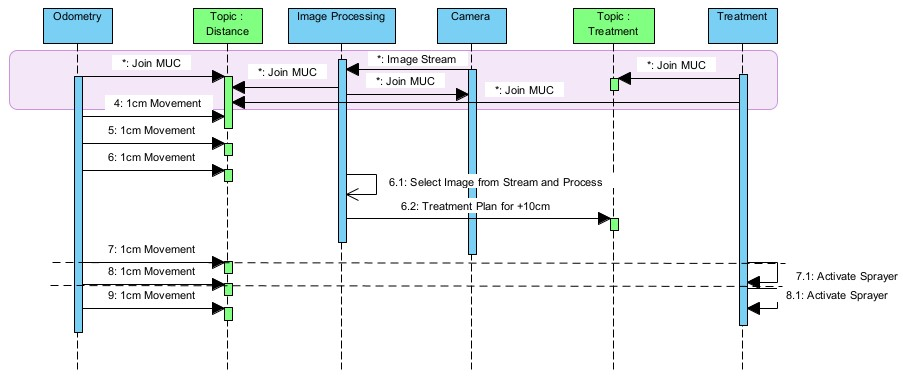
\includegraphics[width=0.75\linewidth]{./figures/uml-system-example.jpg}
	\caption[An example of system conversations]{An example of system conversation---In XMPP based systems, components may simply make announcements (publish) to a Multi-User Chat (MUC, aka chatroom) and components with an interest in those announcements (subscribers) take action. Consider the odometry system. Its sole job is to simply announce that the system has moved forward one unit.}
	\label{fig:uml-system}
\end{figure}

This deployment platform is geared toward optimizing machine learning problems without the overhead of a CPU-based system hosting a GPU.
 
\subsection{Console}
The console is the mechanism for an operator to interact with the system. Figure~\ref{fig:console-operator} illustrates a concept that allows an operator to:
\begin{itemize}
	\item{See the treatment plan currently being applied}
	\item{See the current state of each sprayer}
	\item{See overall statistics for a weeding session}
	\item{Control weeded operations, starting and stopping as required}
\end{itemize}
	

\begin{figure}[H]
	\centering
	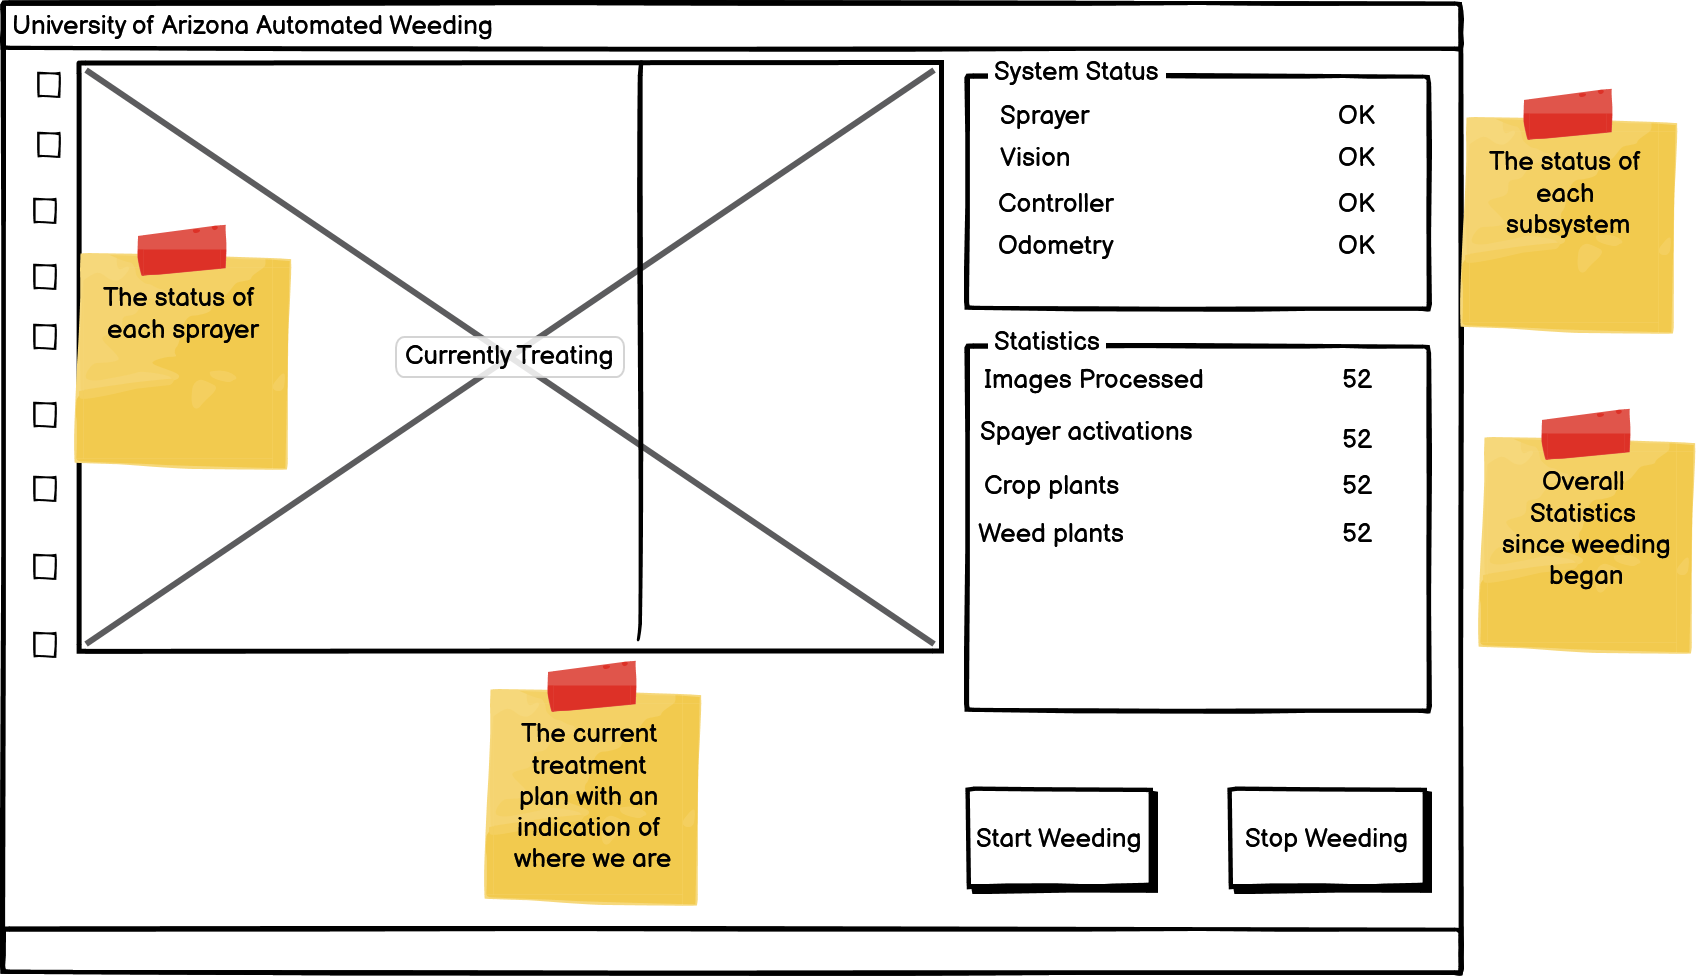
\includegraphics[width=0.75\linewidth]{./figures/console-operator.png}
	\caption[An operator's console]{An operator's console that presents an overview of the current system state. As operators are not concerned with detailed status of system components, the odometry system, for instance, would not appear here.  The console for a system engineer, however, might have a different set of components visible.}
	\label{fig:console-operator}
\end{figure}

While it is unlikely that the final console will take on this exact form, a few guiding principles will guide the final design of this:
\begin{itemize}
	\item{The interface will have as few large controls as possible, for instance large, easily accessed buttons.}
	\item{The interface will be internationalized (I18N), with Spanish and English interfaces the first two languages developed. \footnote{I18N is the process of forming messages that conform to the way users have indicated that they want to receive messages. If they indicate that they want interfaces to be in Spanish, messages are delivered in that form. This does not happen automatically, of course, but the internationalization of an interface must be planned for in an implementation. An oversimplification of this for those familiar with programming is that strings a user see never appear in the code.}}
	\item{The interface will be optimized for use on mobile devices.}
\end{itemize}

Once again, we see an advantage of using a publish-subscribe mechanism of communication. The rest of the system has no knowledge that there is an operator's console, and can be developed without factoring that knowledge that it even exists. That is, the treatment system does not tell the console that sprayer \#4 has been activated, it simply announces that it has activated that sprayer.  The console reports the events it observes in the chatrooms --- chatrooms are where the components of the system carry out conversations about what is the system is doing.

\subsection{Phasing}
This work will be carried out in three phases:
\begin{itemize}
\item{Proof of concept: In this phase some fundamental questions are answered, such as \textit{can weeds and crops be distinguished using visible light images?}}.
\item{Prototype: This phase concentrates on using physical hardware targeted for field use: a camera, an NVIDIA GPU, and a National Instruments Controller. A key question answered in this phase is \textit{can images be processed fast enough to support a commercially viable speed?}}
\item{Production: This phases shifts the focus to the field, where the physical hardware integrated in the previous phase brought together with the existing mechanicals and is proven under real-world conditions.} 
\end{itemize}

\subsubsection{Proof of concept}
This phase will explore and develop the basic approaches to image segmentation and crop/weed discrimination. The target images for this phase will come in two forms: image sets that have been collected in the field, and composed images where various weed placements are tested.
\subsubsection{Prototype}
This phase will integrate software with hardware that will be used in the field, and will integrate with the XMPP communications channel that will be used in the field. The prototype phase will encompass these activities: \\
\begin{itemize}
	\item{Complete the image recognition, odometry, and treatment solution subsystems}
	\item{Integrate with the Basler machine vision camera}
	\item{Port the image processing system to the NVIDIA Jetson and integrate with the hosted GPU}
	\item{Port the odometry system to the National Instruments RIO}
	\item{Port the treatment system to the National Instruments RIO}
	\item{Integrate component communication}
\end{itemize}
\subsubsection{Production}
This phase will have two activities: installation of the physical hardware in the field enclosure, and field testing of the system. This phase will encompass these activities:
\begin{itemize}
	\item{Modify the existing enclosure and install components discussed in Section~\ref{section:system}}
	\item{Field test the integrated system}
\end{itemize}
\subsection{Field Tests}
Field tests will be conducted at the Yuma Agricultural Center of the University of Arizona with the integrates system in two phases: data collection, and wet-runs. Prior to the execution of the data collection phase, however, two calibration activities will be carried out. Once executed, repeating this calibrations will not be required unless there there is a change in any physical equipment (this applies primarily to the vision and odometry subsystems).
\subsubsection{Sensor+Lens Calibration}
The objective of this phase is to determine the pixel to ground distance measurement when the weeding system is in a planting bed deemed 'typical'. This relationship is determined by the following steps\footnote{This calibration may not be required, as the relationship can be determined with some relatively simple equations. The ground sampling distance (GSD) will be $\approx$ \SI{0.02} {\centi\meter} per pixel, a figure that will not vary significantly even when the height of the planting bed varies by a few cm. As this figure far exceeds the precision of the emitter subsystem, it is not anticipated that even a small variation in this figure will have a negative impact on the system.}:
\begin{enumerate}
	\item{A calibration sheet with two green dots centered 4 cm apart is positioned directly beneath one camera}
	\item{Execute a script that will take the image, find the dots, determine the center-to-center distance in pixels. This script will write out a calibration file used by the weeding system}
\end{enumerate}
No forward motion of the weeding system will be required for this stage of the calibration. Calculations or laboratory tests to determine this relationship can be done, of course, but as the distance from the bed to the sensor will likely differ from measurements in the laboratory or used in calculations, this relationship will be determined by this field procedure.  A somewhat related procedure, but one that will be performed under laboratory conditions is the characterization of the distortion introduced by the lens in images of a checkerboard test target. A detailed description of that calibration is beyond the scope of this proposal, but is well documented elsewhere and supported by the OpenCV library set used for various imaging functions.
\subsubsection{Odometry Verification}
The odometry system will be verified on a level, hard, dry surface, under controlled (i.e., enclosed shed or equivalent) using this procedure:
\begin{enumerate}
	\item{A tape measure is placed on the ground along the cropline and extended the length of a planting bed.}
	\item{The weeding system is towed over the entire length at varying speeds including stops an backwards motion.}
\end{enumerate}
This test will compare actual ground distance to the values reported by the system.  As mentioned in Section~\ref{sec:odometry}, it is important that the odometry subsystem be accurate over the distance from the leading edge of the image captured to the emitter line, not accurate over the entire length of the planting bed.
\begin{figure}[H]
	\centering
	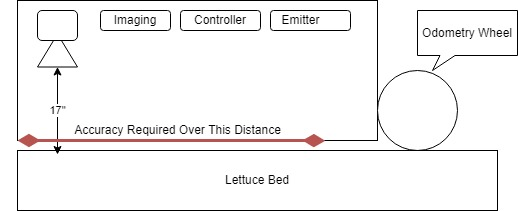
\includegraphics[width=0.75\linewidth]{./figures/odometry-accuracy.jpg}
	\caption[Accuracy required from odometry subsystem]{The odometery subsystem requires accuracy over only a portion of a planting bed, indicated by the red line in this diagram.  The accuracy over this distance must be +/- .5cm, twice the accuracy of the treatment subsystem.}
	\label{fig:uml-system}
\end{figure}
An odometry verification mode of the system software will capture and annotate images, noting every 1cm in forward motion to allow manual verification of accuracy.  Annotated images of the tape are used to verify two things:
\begin{enumerate}
	\item{Image capture accuracy --- Every increment on the tape should be captured, factoring in 20\% overlap at the leading and trailing edges of the image. To correctly classify vegetation that is not fully shown in a single image it will be necessary to stitch adjacent images together.}
	\item{Emitter distance accuracy --- The annotations in the images are not simply markers every 1cm. Rather, the image will be marked with the distance to the leading edge of the image captured by the odometry system.}
\end{enumerate}
\begin{figure}[H]
	\centering
	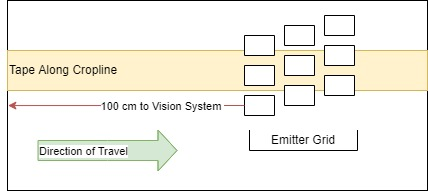
\includegraphics[width=0.75\linewidth]{./figures/test-distance.jpg}
	\caption[Test for distance measurement from emitter]{Note: not to scale. The distance from the center of the emitter to the leading edge of the image captured by the vision system. This figure uses a distance of 100cm only for illustration purposes. The value used will reflect distances in the physical system.}
	\label{fig:test-distance}
\end{figure}

While the absolute accuracy of this odometry system is calculated as noted by this equation:
\begin{align}
\frac {wheel\ circumference}  {rotational\ pulses},\  or\  \frac {92cm} {1000} = .092cm
\end{align}
annotating images with that sort of accuracy would result in too much visual clutter in the resulting image sets.

This procedure will be repeated under field conditions, where wheel slippage is expected to detrimentally affect accurate measurement of distance. Under both conditions, accuracy will be assessed both over the entire distance of a planting bed and over multiples of the distance shown above. These tests will not produce calibration data; their only purpose is to asses and adjust the odometry system.
\subsubsection{Data Collection}
While each run of the system will produce usable data, these "dry" runs will involve only the collection of speed, timing, classification, and imagery. There is no need for a complete and integrated treatment subsystem in these tests, but this phase must be preceded by the calibration tests detailed previously.
 In these runs, the system will collect a series of crop row images, each taken with 20\% front overlap. The image capture strategy reflects a need to stitch consecutive images together before classification, avoiding the problem where the lack of a full view of an object prevents classification. The images collected in this phase will be used for training in future runs, so runs early in this phase are unlikely to be acceptably accurate. Accuracy is expected to improve and will gate the transition to the next phase. Accuracy rates for phase exit will be 3\% false identification of crop as weeds, and 95\% correct identification of weeds as weeds.
The size of the each image set collected in this run will be dependent on several factors:
\begin{enumerate}
	\item{The size of the Region of Interest (ROI) --- the vision system proposed for this project (Basler) supports the notion of an ROI that may be a subset of the full capability of the sensor. Suppose that a strip above and below the crop line can be ignored. Capturing and processing this information may not be worthwhile.}
	\item{The compression rate of the camera system --- there is a tradeoff between image quality and the amount of compression applied. A 5 mega-pixel image contains 15 MB of data, but may be only 1 MB after compression. The image produced by the Basler acA1920-gc camera, for instance is 452 KB.}
	\item{The ground distance captured in each image}
	\item{The length of each planting bed row and the number of rows}
\end{enumerate}
Each image footprint is dependent on selections made for the vision subsystem. Using the values for a Basler acA1920-gc with a 5mm focal length lens\footnote{This camera was the only one available to the author at the time of this writing, and may not be chosen for the final project}, the image captured has these characteristics:
\begin{align}
	x = \left( \frac {elevation} {focal\ length} \right) \ *\ sensor\ width,\ or\ \left( \frac {502mm} {5mm} \right) 4.2mm = \SI{437.388}{\milli\meter} \\
	y = \left( \frac {elevation} {focal\ length} \right) \ *\ sensor\ height,\ or\ \left( \frac {502mm} {5mm} \right) 2.4mm = \SI{240.960}{\milli\meter}
\end{align}
The length of the planting bed and number of rows is variable, of course, but this proposal will assume there are four rows, each 20m in length. The total number of images is given by:
\begin{align}
	images = \frac {4 * 20m * \frac{1000mm} {1m}} {437.388mm * .8} = 228.63
\end{align}
The space needed for a single image capture set is:
\begin{align}
229\ images * \frac{\SI{452}{\kilo\byte}} {image} \approx \SI{103.5}{\mega\byte}
\end{align}

A \SI{64}{\giga\byte} flash drive on the Jetson will provide a minimum of \SI{40}{\giga\byte} of free space, enough for several image collections. It is not anticipated that this space will be used, however, as image sets will be automatically uploaded to CyVerse (for off-line analysis; this activity is not real-time) and deleted from local media upon the completion of a run and IP connectivity to CyVerse can be established.

\subsubsection{Wet-Run} 
This phase requires all subsystems to be functionally complete and integrated. During these runs, the identified weeds are treated with a tinted, non-toxic liquid.  Treatment efficacy and accuracy can be assessed in two ways:
\begin{enumerate}
	\item{Manually, by assessing the coverage of each plant by the treatment --- a manual assessment has the advantage of detailed inspection of each application, but suffers from the inevitable errors in any manual assessment.}
	\item{Automatically, by capturing images of post-treatment vegetation --- This approach would processes post-treatment images either by capturing images in real-time after treatment or by performing an additional dry-run immediately after a treatment, collecting an image set that can be used.  Collection of images immediately after treatment would require a new set of cameras immediately after the treatment system, a requirement that may not be mechanically feasible due to physical space constraints. The additional dry-run approach will be used in this project.}
\end{enumerate}
The automatic assessment of spray requires an image segmentation geared toward the hue of the dye, allowing the separation of treated vegetation. Once segmented, each unwanted plant is scored based on the percentage of leaf area treated. Once sufficient accuracy is achieved, treatment will transition from dyed water to dyed herbicide. Until that accuracy in achieved, weeds will be treated by manual remediation. Treatment accuracy should not be conflated with classification accuracy. While the classification of vegetation is an indication of the fate of a plant (treated or not, the intent), treatment accuracy is an indication of what actually happened. In practice, of course, the treatment accuracy will be 100\%, even if the classification is incorrect.


 \newpage
%
% W E A K N E S S E S
%
\section{Weaknesses of Study}
This proposal has weaknesses in four areas: weed/crop discrimination under field conditions, weed/crop discrimination over the growth cycle, system redundancy, and information security.

\subsection{Weed/Crop Discrimination Under Field Conditions}
While the concepts around this are explored in the proof of concept phase, the image sets used there are obtained under lighting conditions that will  not be encountered in the production phase. The structural features noted previously will probably be invariant to changes based on lighting -- how round an object is does not depend heavily on lighting conditions, for instance. Color features, however, may. Vegetation may exhibit different responses to LED light than to full-spectrum sunlight. If this is encountered, we plan to deal with this by either adjusting the aforementioned thresholds applied to a vegetation index, or to use an index more suited to the spectrum encountered.

%\subsection{Weed/Crop Discrimination over the Grown Cycle}

\subsection{Redundancy}
The system described in this proposal has multiple single points of failure. In such a system, for instance, the failure of a shared resource -- such as the National Instruments RIO controller -- would render the entire system unusable. The failure of a resource dedicated to a task, but with a peer performing the same task -- such as processing the images along the right side of a row -- will result in the degradation of system, but not a complete failure.
\begin{figure}[H]
	\centering
	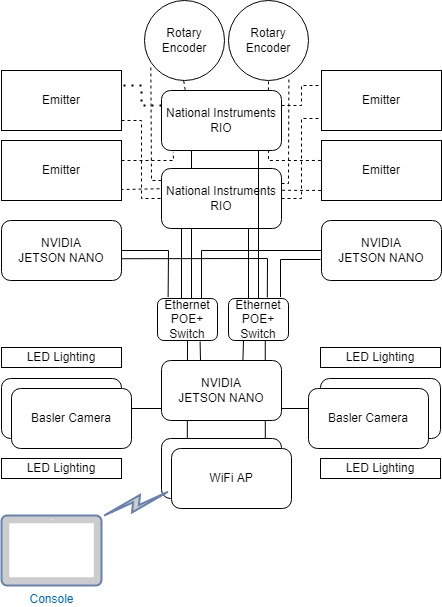
\includegraphics[width=0.4\linewidth]{./figures/system-overview-Page-2.jpg}
	\caption[An overview of a redundant system]{An overview of a redundant system, illustrating that there is no single point of failure}
	\label{fig:system-overview-redundant}
\end{figure}

Figure~\ref{fig:system-overview-redundant} illustrates a system without a single point of failure. If a RIO controller fails, for example, the system can use the redundant controller. If an Ethernet switch fails or if a cable fails connecting a component, that component can use the redundant network. In these systems, there are redundancy decisions that can be made locally -- a link to a switch has failed and the other switch must be used --- and redundancy decisions that must be made system-wide -- the failure of a component hosting the messaging server, for instance. That the system shows three NVIDIA devices is indicative of the N+1 redundancy scheme used by such a system. This system can tolerate the loss of only one NVIDIA, as it must have a \textit{quorum} of members to form a redundancy group. It is beyond the scope of this proposal to discuss redundancy schemes in depth, and the overly broad statements here are not meant to be an analysis of failure scenarios. \\
For the proposed system, we will characterize the risk by computing MTBF of the physical components (these may not be available for components, but are typically supplied by the vendor).  While it does not mitigate the risk, system components will perform extensive self-tests when the system is first brought up, as well as non-invasive self tests during system operation. These self test results will speed the identification of faulty components, leading to higher uptimes and simplifying field deployments.
 
\subsection{Information Security}
This proposal does not address the information security of the system, and a full assessment of that topic is beyond the scope of this document. While this system does not control a high-value target, the opportunities for compromising the subsystems can not be ignored entirely. The final system will take some best-practices approach to system components:
\begin{itemize}
	\item{Minimize the attack surface by shutting down unneeded services}
	\item{Using certificates in lieu of passwords for establishing communication}
	\item{Encrypting all communications between components}
	\item{Scanning the system with penetration testing software}
\end{itemize}


%\newpage
%\section{Public Health Significance}
 
%\section{Budget}
%\label{section:budget}
%Table~\ref{table:budget} reflects the total expenditures involved in this study. While not broken down by year, it is anticipated that these expenditures will take place over two years. Amounts specified are in US\$.
%\begin{table}[h]
%\centering
%\begin{tabular}{lrlr}
% 	\toprule
%	Salaries/Wages    &  & 2670.60 \\
%	\midrule
%	& Mechanicals & 1965.00 \\
%	&Field Operator & 705.60 \\
%	\midrule
%	Travel & & 2241.72 \\
%	\midrule
%	& In State & 2241.72 \\
%	\midrule
%	Supplies & & 6789.00 \\
%	\midrule
%	\midrule
%	Project subtotal & & 11701.32 \\
%	\midrule
%	Indirect Costs (53\%)\tablefootnote{This may not be required if separate funding is not obtained. If that is not the case, the project subtotal should be considered the grand total for the project.} & & 6201.70 \\
%	\toprule
%	\toprule
%	\textsc{Total Project}                      & & \underline{18387.92} \\
%
%	\bottomrule
%    \bottomrule                
%\end{tabular}
%\caption[Total Budget Breakdown]{A breakdown of expenditures for this study}
%\label{table:budget}
%\end{table}
%
%%
%% S A L A R I E S
%%
%\subsection{Salaries and Wages}
%Table~\ref{table:salaries} reflects the salary expenditures for this study.  The components discussed in Section~\ref{section:system} will need to be installed in the existing enclosure. To accommodate these components, mechanical modifications will be required and will be carried out at the Yuma Agricultural Research Center. Once a modified system is ready, an operator qualified to operate a tractor in a field setting will conduct test runs using the system at the Valley Farm site of the Yuma Agricultural Research center.
%\begin{table}[H] % Force the table to show below the paragraph
%\centering
%\begin{tabular}{lrlrlrlrlrlrlr}
% 	\toprule
%	Role & Per Hour & Hours Per Week & Weeks & ERE & Subtotal \\
%	\toprule
%	Mechanicals & 25.00 & 20 & 3 & 31.0\% & 1965.00 \\
%	Field Operator & 15.00 & 2 & 20 & 17.6\% & 705.60 \\
%	\toprule
%	\toprule
%	\textsc{Total Salaries} & & & & & \underline{2670.60} \\
%
%	\bottomrule
%    \bottomrule                
%\end{tabular}
%\caption[Salary Breakdown]{A breakdown of salaries for this study}
%\label{table:salaries}
%\end{table}
%
%%
%% T R A V E L
%%
%
%\subsection{Travel}
%Travel funds dedicated for in-state travel represent 6 trips to Yuma, Arizona to oversee physical system integration of the automated system and to oversee and collect data from field trials. These activities both take place at the University of Arizona Yuma Agricultural Center.
%\begin{table}[H] % Force the table to show below the paragraph
%\centering
%\begin{tabular}{lrlr}
% 	\toprule
%	\toprule
%	6 Trips to Yuma, AZ & & 2241.72 \\
%	\midrule
%	& Vehicle Rental for 2 days per trip @ \$67.31 & 1407.72 \\
%	& Lodging for 1 day per trip @ \$94.00 & 564.00 \\
%	& M\&IE for 2 days per trip @ \$45.00 & 270.00 \\
%	\toprule
%	\toprule
%	\textsc{Total Travel}                      & & \underline{2241.72} \\
%	\bottomrule
%    \bottomrule                
%\end{tabular}
%\caption[Travel Budget Breakdown]{A breakdown of travel expenditures for this study}
%\label{table:travel}
%\end{table}

%
% S U P P L I E S
%
\section{Supplies}
\label{section:supplies}
Table~\ref{table:supplies} reflects the supply expenditures for this proposal. All of the supplies here represent the Bill of Materials (BOM) of the final system, and will be installed in the existing enclosure. These supplies are required to support the completion of the \textit{deployment} phase detailed in Section~\ref{section:phases}.\\

\begin{table}[H] % Force the table to show below the paragraph
\centering
\begin{tabular}{lrlr}
 	\toprule
 	Item & Quantity & Price \\
 	\midrule
	Heavy Duty TRD-GK Rotary Encoder & 1 & 269.00 \\
	NVIDIA Jetson & 2 @ 459 &918.00 \\
	NVIDIA Jetson Enclosure &2 @ 25 & 50.00 \\
	LED Lamps & 4 @ 150 & 600.00 \\
	National Instruments CompactRIO&1& 1567.00 \\
	9411 Module for RIO &1& 372.00 \\
	9403 Module for RIO &1& 656.00 \\
	Cables &6+& 75.00 \\
	Basler ACE2 Machine Vision Camera &2 @ 730& 1460.00  \\
	Computar C-Mount Lens &2 @ 320& 640.00 \\
	POE+ Ethernet Switch &1& 50.00 \\
	WiFi Outdoor Access Point &1& 70.00 \\
	Encoder Power Supply &1& 12.00 \\
	NVIDIA Jetson Power Supply &2 @ 25& 50.00 \\
	\midrule
	\midrule
	\textsc{Total Supplies}                      & & \underline{6789.00} \\
	\bottomrule
    \bottomrule                
\end{tabular}
\caption[Supply Budget Breakdown]{A breakdown of supply expenditures for the deployment stage of this study}
\label{table:supplies}
\end{table}




%\end{table}

%REFERENCES
%Use the Vancouver Style of referencing. This is found at this website:
%http://www.ncbi.nlm.nih.gov/books/bv.fcgi?rid=citmed.TOC&depth=2 or a less detailed website:
%http://www.nlm.nih.gov/bsd/uniform_requirements.html
%
%References should be numbered consecutively in the order in which they are first mentioned in the text. Identify references in text, tables, and legends by Arabic numerals in parentheses. The titles of journals should be abbreviated according to the style used in Index Medicus. Consult the list of Journals Indexed for MEDLINE, published annually as a separate publication by the National Library of Medicine. The list can also be obtained through the Library's web site..



 


% 
% E N D  T E M P L A T E  F R O M  W O R D
%

\newpage
{
\setstretch{1.0}
\section{References}
\printbibliography[heading=none]
}

\end{document}

